% Objective of the paragraph: setup the hype context and importance of the problem
Reinforcement learning (RL) allows for agents to learn complex behaviors
in a multitude of environments while requiring supervision only in the
form of reward signals. RL has had success in various domains ranging
from playing Atari games~\citep{MnKaSiNATURE2015} from purely visual
input and defeating world GO champions~\citep{gibney2016google}, to
applications in robotic navigation~\citep{mirowski2018learning} and
manipulation~\cite{levine2018learning}. In the realm of multi-goal tasks,
this work introduces Floyd-Warshall Reinforcement Learning (FWRL), a new
algorithm that facilitates the transfer of learned behaviours in
environments with dynamic goal locations.


% brief background on model-based and model-free learning.
There are two types of RL algorithms, \emph{model-based} and
\emph{model-free}, which differ in whether the state-transition function
is learned explicitly or implicitly~\citep{SuBaBOOK1998}.  In
\emph{model-based} RL, the dynamics that govern an environment's
transitions is explicitly modelled.  At any point in an episode, agents
use this model to predict future states and utilize this information to
maximize possible reward. This formulation is known to be
sample-efficient while normally not achieving high asymptotic
performance~\citep{pong2018temporal}.  In contrast, in \emph{model-free}
RL, algorithms such as policy gradients, actor-critic and Q-learning
directly learn the expected ``value'' for each state without explicitly
learning the environment-dynamics. This paradigm has been behind most of
the successes in such diverse applications
like Atari games, Go championships etc.

\begin{figure}%
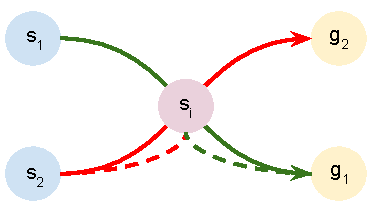
\includegraphics[width=\columnwidth]{./media/optimal_trajectories.pdf}\\
\caption{The intuition driving Floyd-Warshall Reinforcement Learning.
Consider an agent experiencing traversals from $s_1$ to $g_1$ and then from
$s_2$ to $g_2$. Assume that there is at least one common state $s_i$ in
the two trajectories. The agent is then directed to traverse to $g_1$ from
$s_2$. The agent can \emph{exploit} previous trajectories to find a path to
perform this traversal (the dotted line), without requiring extensive
\emph{exploration}. However, standard Q-Learning cannot
make these generalizations. FWRL utilizes a triangle-inequality like constraint
(Eq~\eqref{eq:fwconstraint}) to combine trajectories from past experiences.
}
\label{fig:visual-abstract}%
\end{figure}

% Goal-conditioned tasks
%Many problems in robotics, like navigation, and  pick and place tasks
%can be formulated in multi-goal domains where the task to be completed
%requires the specification of goal information. However, for such tasks
In multi-goal tasks that involve static environments and dynamic goals,
such as goal-directed navigation and pick-and-place in robotics,
model-free RL struggles to transfer learned behavior from one goal
location to another within the same
environment~\citep{dhiman2018critical,quillen2018deep}. This occurs because model-free
RL represents the environment as value functions, which conflate the
state-dynamics and reward distributions into a single representation.
On the other hand, model-based RL allows for the separation of
environment dynamics and reward, but can have lower asymptotic
performance due to the accumulation of small errors in the modelling function.

In this work we introduce Floyd-Warshall Reinforcement Learning, an
adaptation of the Floyd-Warshall shortest path
algorithm~\citep{floydwarshall1962}, for multi-goal tasks.
The Floyd-Warshall shortest path algorithm is itself a generalization of
Dijkstra's algorithm for multi-goal domains on graphs. The algorithm works
by learning a goal conditioned value function
~\citep{schaul2015universal}, called the Floyd-Warshall (FW) function,
that is defined to be the expected reward in going from a start
state-action pair $(\state, \act)$ to a given goal state $\state'$:
%
\begin{align}
\fwargs{\state}{\act}{\state'}{\policy}{} =
\E_{\policy}\left[ \sum_{t=0}^{t=k} \rew_t \middle\vert \state_0 = \state, \act_0 = \state, \state_k = \state' \right] .
\end{align}%
%
In order to learn the FW-function, we employ the following
triangular-inequality constraint for shortest paths, which is our main
contribution,
%
\begin{multline}
\fwargs{\state_i}{\act_i}{\state_j}{\policy^*_{\state_j}}{*}
 \ge 
  \fwargs{\state_i}{\act_i}{\state_k}{\policy^*_{\state_k}}{*}
  + \max_{\act_k}\fwargs{\state_k}{\act_k}{\state_j}{\policy^*_{\state_j}}{*}
  \\
  \forall \state_k \in \State.
  \label{eq:fwconstraint}
\end{multline}%
%
Section~\ref{sec:method} describes the terminology, equations and the method in more detail.

This constraint allows FWRL to remember paths even if they do not lead
to the goal location during particular episodes. The motivation is
similar to the Hindsight Experience Replay
(HER)~\citep{anderson2017vision}, where agents learn by re-imagining the
final states of past failed experiences as succesful. Our method allows
us to utilize hindsight experience in more a fine-grained manner because
we consider all states as potential goals. Other works using a
goal-conditioned value function for multi-goal tasks include Universal
Value Function Approximators (UVFA)~\citep{schaul2015universal} and
Temporal Difference Models (TDM)~\citep{pong2018temporal}. UVFA
introduces the use of goal-conditioned value functions and a
factorization approach for faster learning of neural networks that
depend upon goals from the state space.  TDM combines model-based and
model-free algorithms by modeling the learning as a constrained
objective function using a horizon dependent goal-conditioned value
function. In contrast to these works, we present an alternative
mechanism for learning these functions that is horizon independent.  

Experimentally, FWRL is shown to be more sample-efficient and achieve higher
reward standard Q-Learning and model-based methods in a tabular setting. FWRL is
found to achieve two times median rewards than the next best baseline.


%Recently, a few works have used the idea of goal-conditioned value functions. In
%Temporal-Difference modelling \cite{pong2018temporal} model a goal conditioned
%action-value function that is also conditioned on the horizon. In contrast our
%proposed value function is independent of horizon length, and hence easier to
%estimate.


\section{Hindsight Experience replay}

Works by sampling sub-trajectories from past episodes and resampling rewards

\section{Different components of loss function}
